\section{Conclusione}

Gli obiettivi prefissati all'inizio dell'esperienza sono stati raggiunti con successo. Lo studio della calibrazione ha permesso di valutare quantitativamente il contributo della strumentazione utilizzata durante la presa dei set di dati, nel corso dell'esperienza.
\\\\
Un corretto svolgimento di essa ha portato a una soddisfacente analisi  riguardante la regione dell'idrogeno, in particolare l'emissione della riga H21.
I risultati finali sono stati ottenuti tenendo conto delle considerazioni sull'effetto Doppler e sul moto di rivoluzione terrestre.
\\\\
Mettici 30 e Lode grazi tesoro.

\begin{figure}[H]
	\centering
	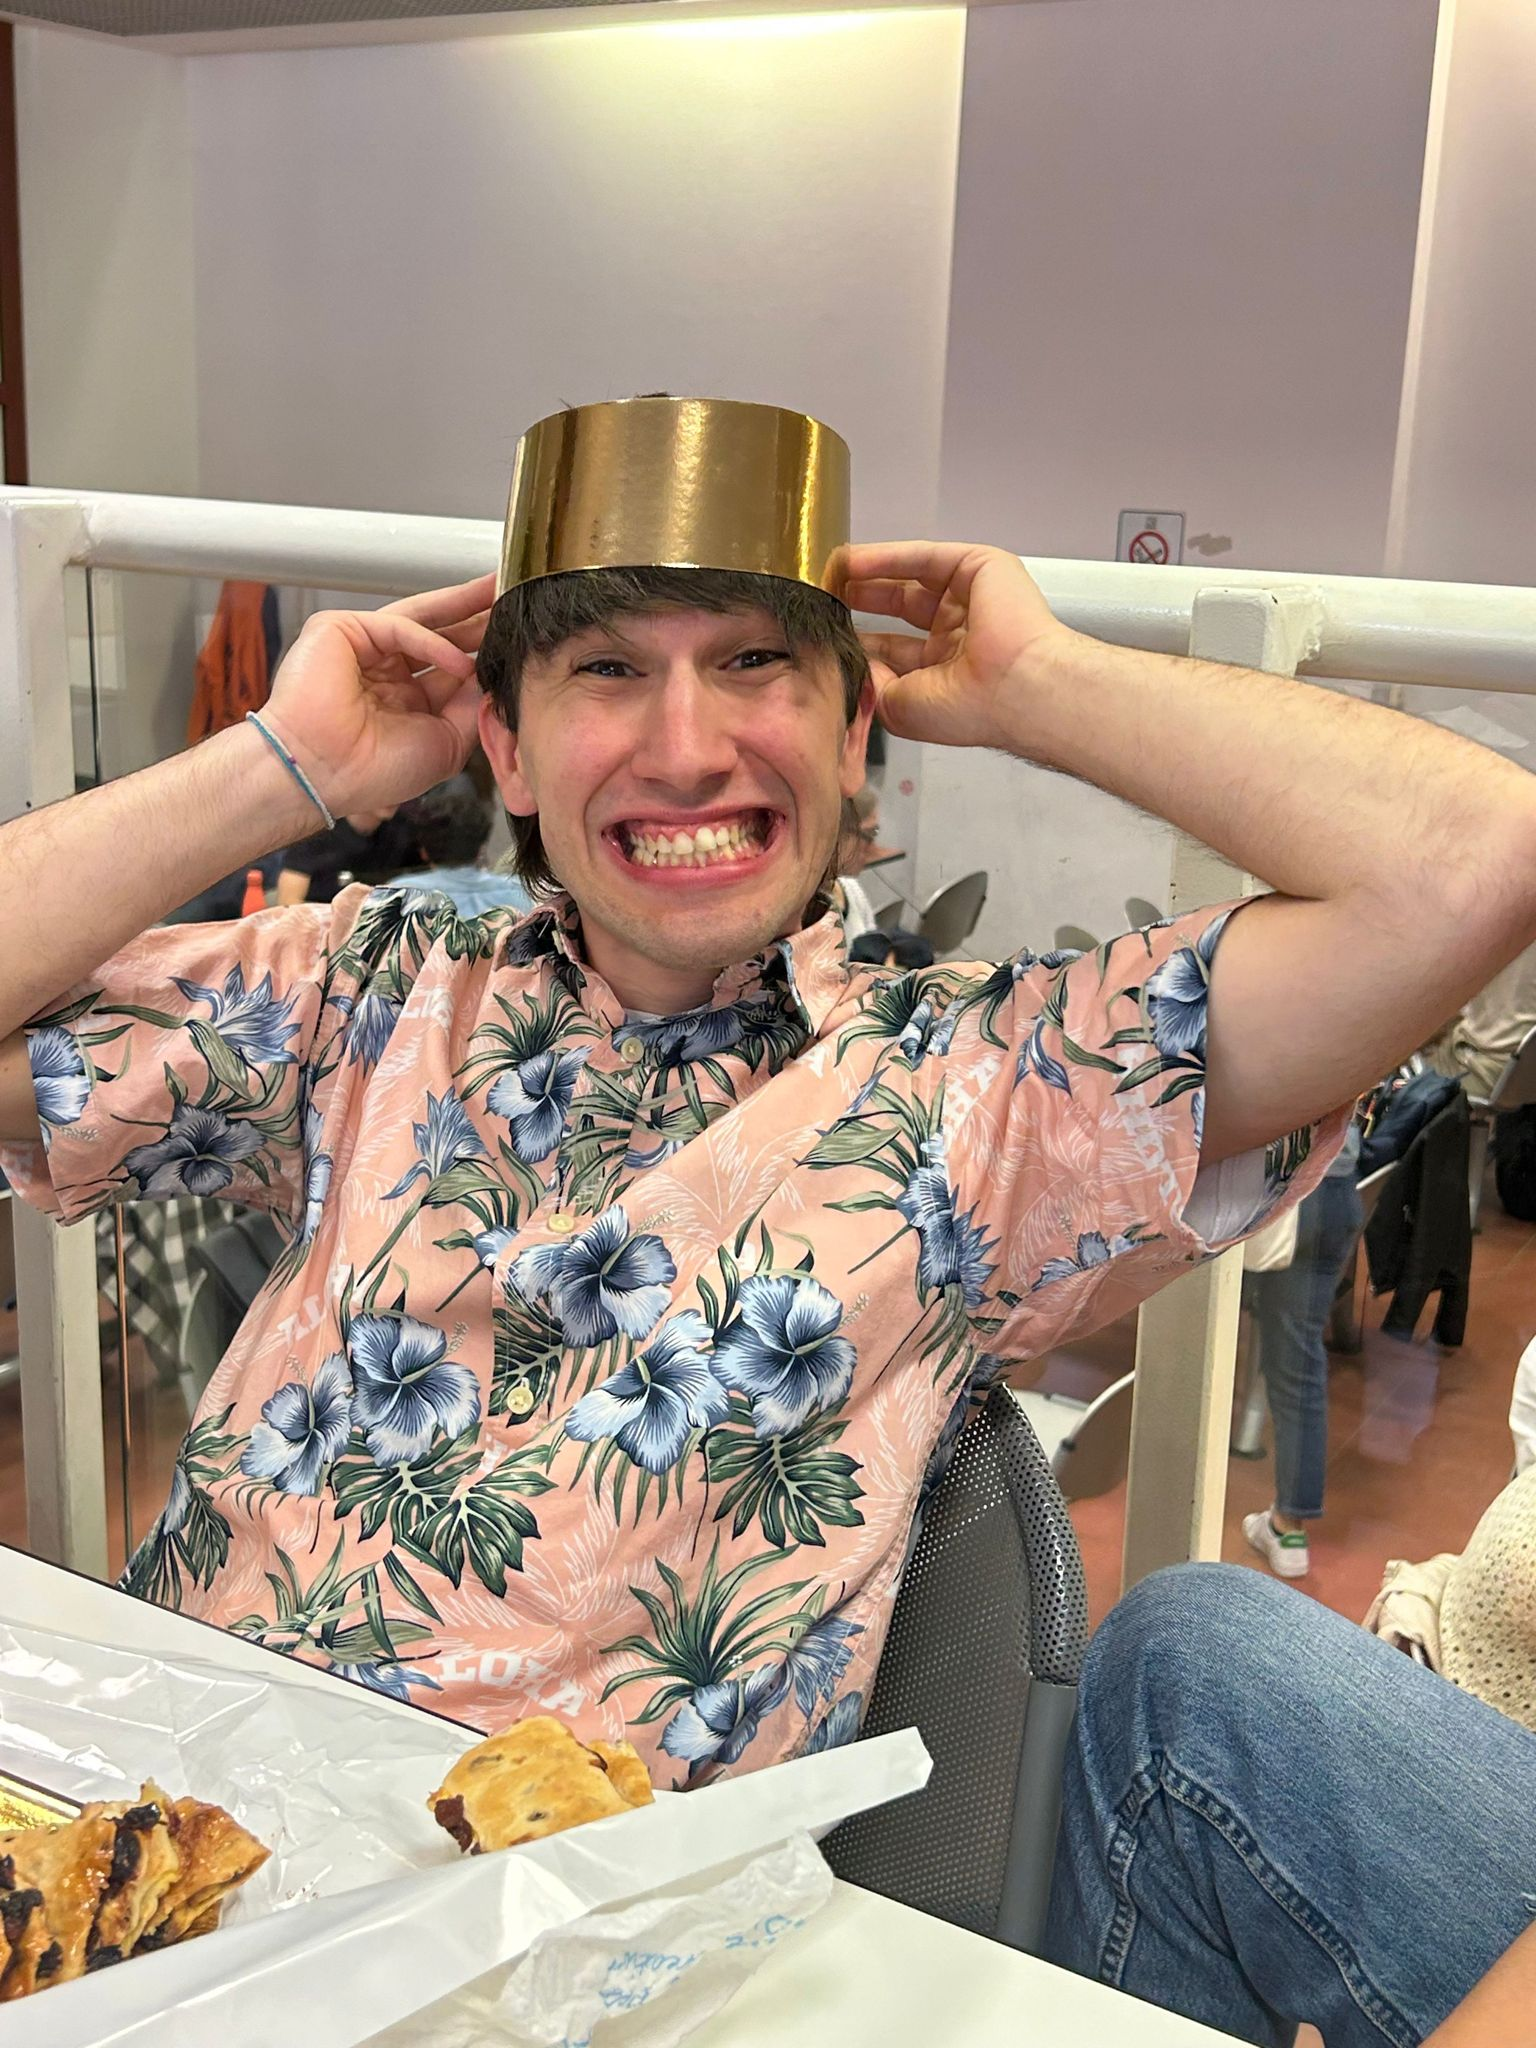
\includegraphics[scale=0.1]{Mapp_cigno_2.jpeg}
	\caption{Il nostro Cigno}
    	\label{fig:Mappa_finale}
\end{figure}